\documentclass[14pt]{article}

\usepackage[a4paper, portrait, margin=1.5cm]{geometry}

%Russian-specific packages
%--------------------------------------
\usepackage[T2A]{fontenc}
\usepackage[utf8]{inputenc}
\usepackage[russian]{babel}

\usepackage{amssymb}
\usepackage{mathtools}

\usepackage{centernot}
\usepackage{stmaryrd}
\usepackage{amsthm}
\usepackage{amsmath}
\usepackage{graphicx}


%--------------------------------------
 
%Hyphenation rules
%--------------------------------------
\usepackage{hyphenat}
\hyphenation{ма-те-ма-ти-ка вос-ста-нав-ли-вать}

\title{Домашнее задание 1 по предмету "Методы оптимизации"}
\author{ Михаил Лобанов, Б05-926 } 

\newtheorem*{details}{Пояснение}

\graphicspath{ {./images/} }

\begin{document}
\maketitle

\section{Теоретические результаты}
В рамках решения задачи о логистической регрессии мы минимизируем следующую функцию:
\begin{equation}
	f = \frac{1}{m}\sum_{i=1}^m\ln \Big(1 + \exp{(-b_i, \langle a_i, x \rangle)}\Big) + \frac{\lambda}{2} \|x\|_2^2 \xrightarrow[x \in \mathbb{R}^n]{} \min
\end{equation}
Градиент и гессиан выражаются следующим образом:

\begin{equation}
	\nabla{f} = \lambda \cdot x - \frac{1}{m} A^T(b \cdot \frac{1}{1 + \exp{(b^T \cdot Ax)}})
\end{equation}

\begin{equation}
	\nabla^2{f} = \frac{1}{m}A^T\frac{1}{1 + \exp{(b^T \cdot Ax)}}(1 - \frac{1}{1 + \exp{(b^T \cdot Ax)}})I_nA + \lambda \cdot \mathit{I}_n
\end{equation}

Функция в матрично-веткорной форме

\begin{equation}
	f = \frac{1}{m} \Bigg\langle 1_m,  \ln \Big(1 + \exp{(-b \odot Ax)}\Big) \Bigg\rangle + \frac{\lambda}{2} \|x\|_2^2
\end{equation}

\begin{details}
	\textrm{Размерности} $ b \mapsto (m, 1), A \mapsto (m, n), x \mapsto (n, 1).$
\end{details}

\section{}
\section{Эксперименты}

\subsection{Траектория градиентного спуска на квадратичной функции}

Градиентный спуск чувствителен к сжатию осей. Рассмотрим две квадратичных функции, одна с обычными осями, а другая - "сплюснутая".

\begin{figure*}[h]
	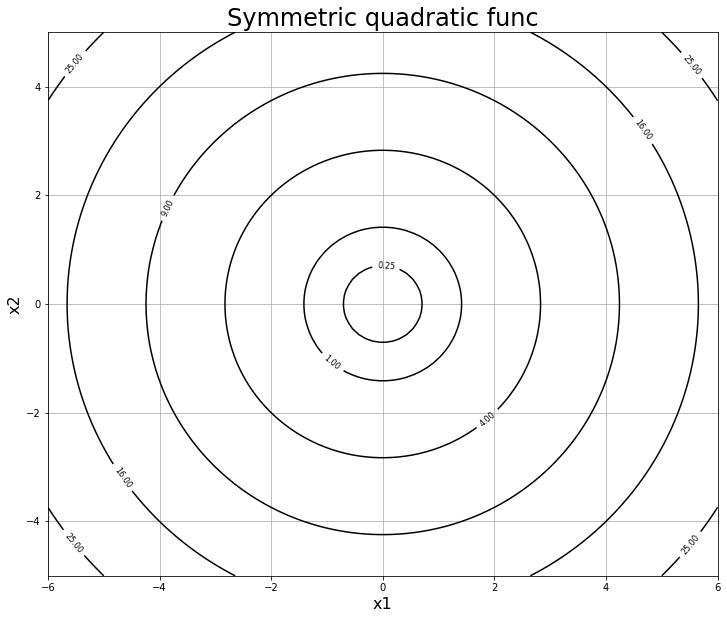
\includegraphics[width=0.5\textwidth]{sym_simple.png}
	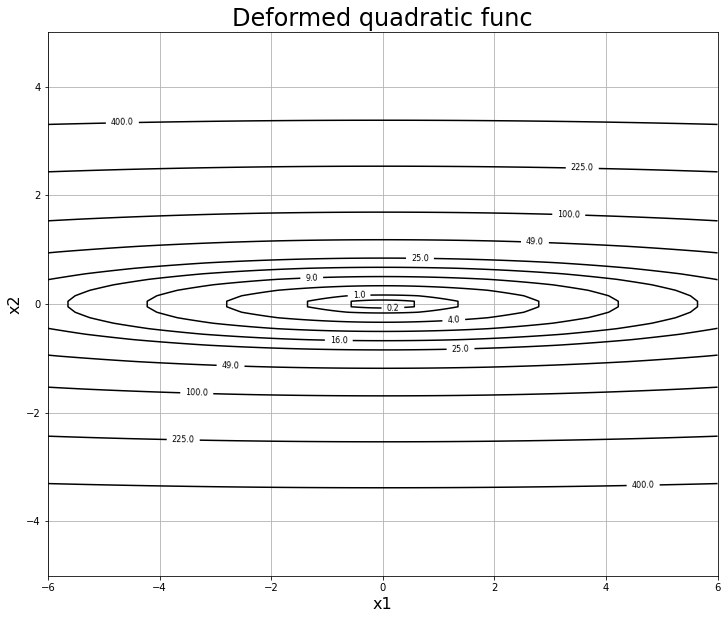
\includegraphics[width=0.5\textwidth]{deformed.png}
\end{figure*}

\newpage

\textbf{Симметричная функция.}
С ней справляется градиентный спуск в любой модификации: и с константным подбором шага, и с правилом Вульфа, и с правилом Армихо. Разве что в константном случае шагов требуется много.

\begin{figure*}[h]
\centering
	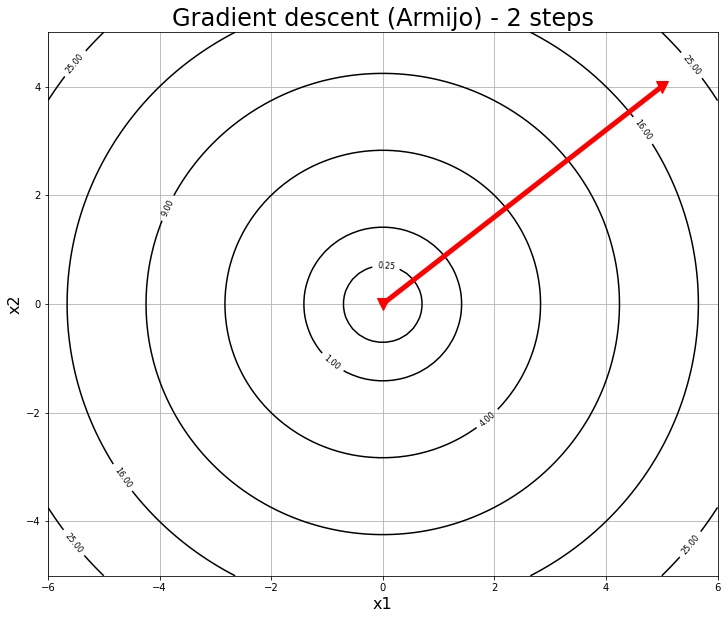
\includegraphics[height=6.7cm]{sym_armijo.png}
	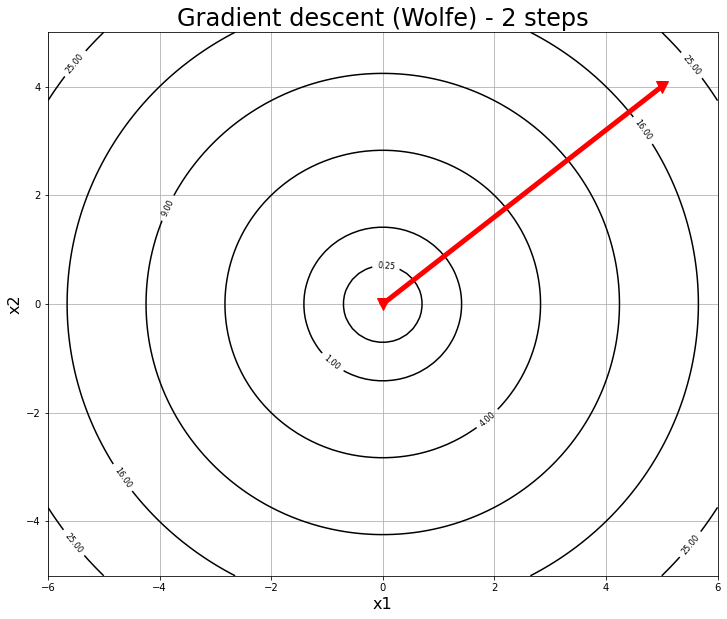
\includegraphics[height=6.7cm]{sym_wolfe.png}
	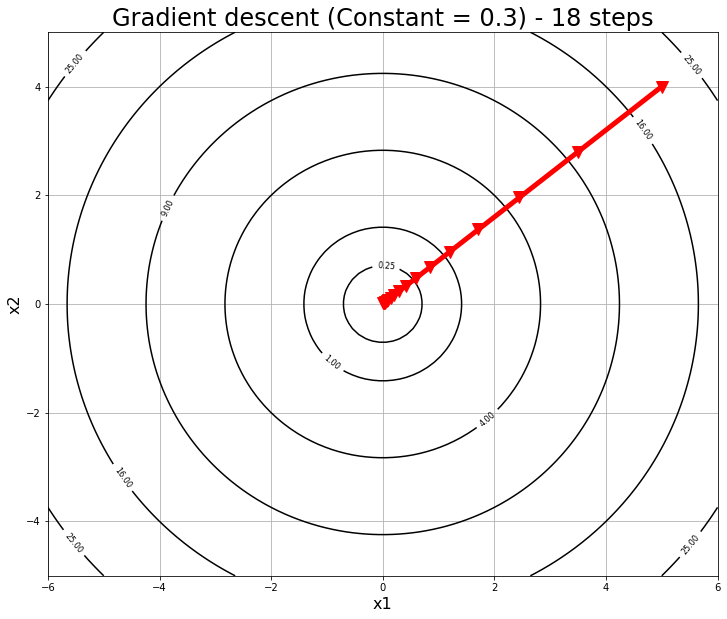
\includegraphics[height=9cm]{sym_const.png}
\end{figure*}

\newpage


\textbf{Сжатые оси.} При деформации осей алгоритм начинает работать сильно хуже. На соответствующей функции GD с Армихо стал "петлять" из стороны в сторону, GD с константным шагом вообще не получилось свести, и только Вульф показал себя хорошо.

\begin{figure*}[h]
\centering
	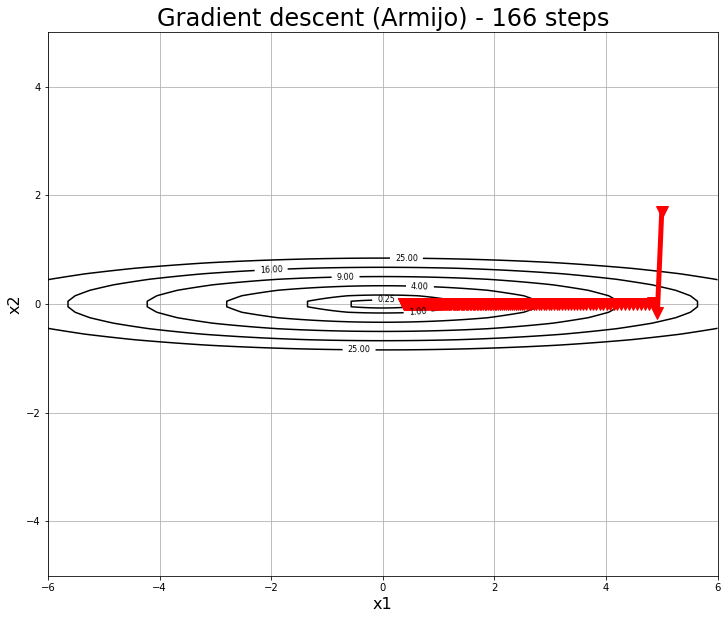
\includegraphics[height=0.256\paperheight]{deform_armijo.png}
	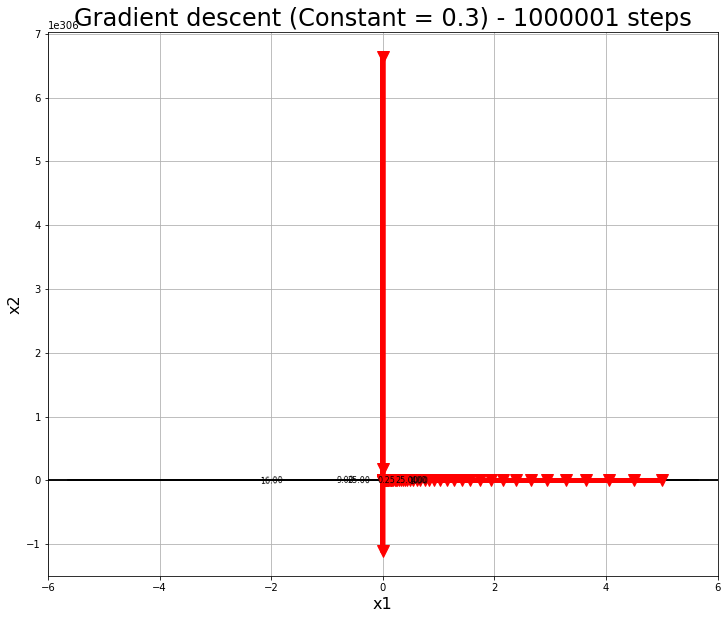
\includegraphics[height=0.256\paperheight]{deform_const.png}
	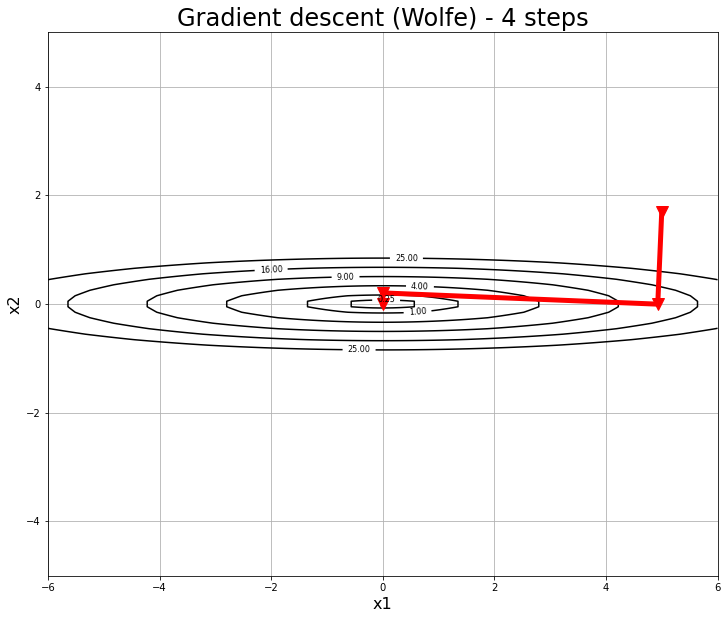
\includegraphics[height=0.4\paperheight]{deform_wolfe.png}
\end{figure*}

Эксперименты показали, что нет качественной зависимости между сходимостью и начальной точкой (либо из всех сходится, либо из всех не сходится). Видимо поэтому начальную точку часто выбирают случайно.

\newpage

\subsection{Зависимость числа итераций градиентного спуска от числа обусловленности и размерности пространства
}

\\

Рассмотрим 4 различных размерности $n$: $[10, 10^2, 10^3, 10^4]$ и 49 чисел обусловленности $\kappa$: от 2 до 49 включительно. Для каждой пары $(n, \kappa)$ сформулируем 100 задач минимизации квадратичной функции размерности $n$ и числом обусловленности $\kappa$.  
\\ \\ Решим каждую задачу и подсчитаем количество итераций $T_i(n, \kappa), i \in \{1, \dots, 100\} $, которое прошел GD номер $i$. \\ \\
Посмотрим на среднее количество итераций при каждом $\kappa$ и $n$:

\begin{figure*}[h]
	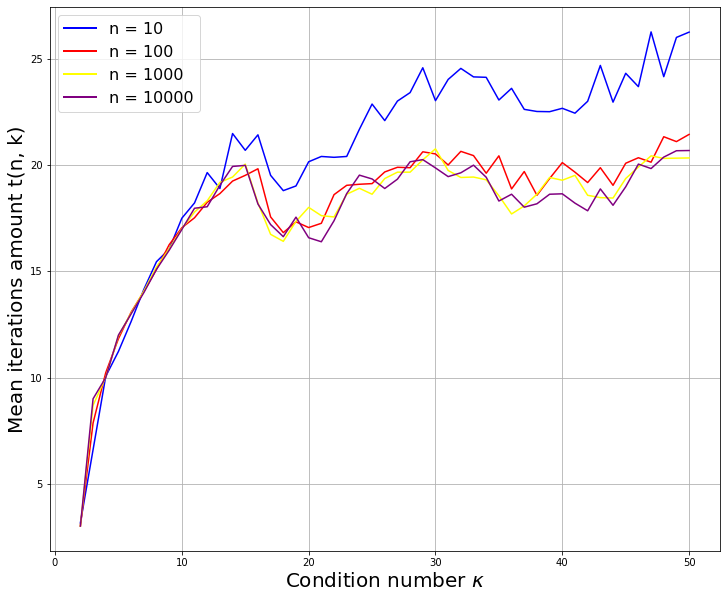
\includegraphics[width=\textwidth]{mean_kappa.png}
\end{figure*}

 Видим, что примерно до $n = 15$ есть четка корреляция между числом обусловленности и количеством итераций. После зависимость перестает быть такой ясной.
 
 \newpage
 
 Нанесем на график вообще все результаты эксперимента:
 
\begin{figure*}[h]
	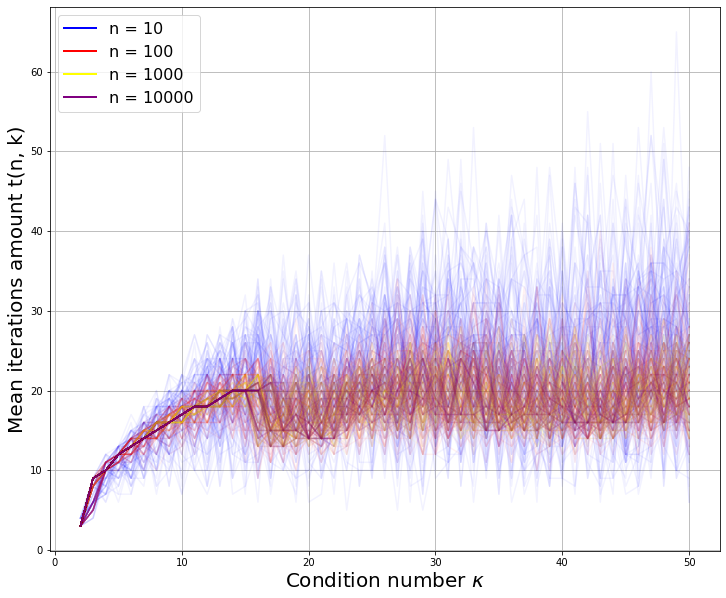
\includegraphics[width=\textwidth]{all_kappa.png}
\end{figure*}

График наталкивает на мысль, что чем больше размерность, тем меньше дисперсия количества итераций, а чем больше $\kappa$, тем она выше. Проверим:

\begin{figure*}[h]
	\centering
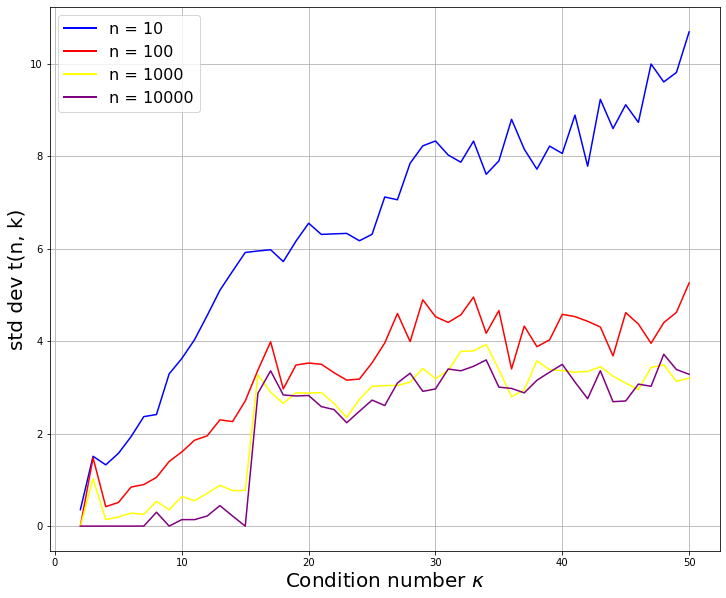
\includegraphics[height=5.2cm]{stddev_kappa.png}
\end{figure*}


Действительно, график стандартного отклонения показывает, что чем больше $\kappa$, тем больше разброс в количестве итераций GD. И чем меньше размерность, тем это виднее.



\newpage



\subsection{Сравнение методов градиентного спуска и Ньютона на реальной задаче логистической регрессии}

Все три датасета (w8a, gisette, real-sim) приводят к следующим выводам:
\begin{enumerate}
	\item Метод Ньютона сходится гораздо быстрее, чем метод градиентного спуска: требуется меньше итераций, со временем (по мере спуска) GD теряет эффективность сильнее, чем NM.
	\item Метод Ньютона сильно более затратный. На одну итерацию требуется больше времени и памяти.
	\item Иногда NM невыгоден, поскольку хоть и сходится быстро, но слишком медленно. Пускай GD и делает в разы больше итераций, но он делает их за секунды.
	\item Нормированный градиент убывает очень похоже на значение самой функции с точностью до масштаба.
\end{enumerate}
	\\ \\ Далее приведем графики экспериментов. 

\newpage

\vspace{20pt} \textbf{Датасет w8a}.

Зависимость значения функции от времени, от масштабированного времени (на отрезок $[0, 1]$), от номера итерации.


\begin{figure*}[h]
	\centering
	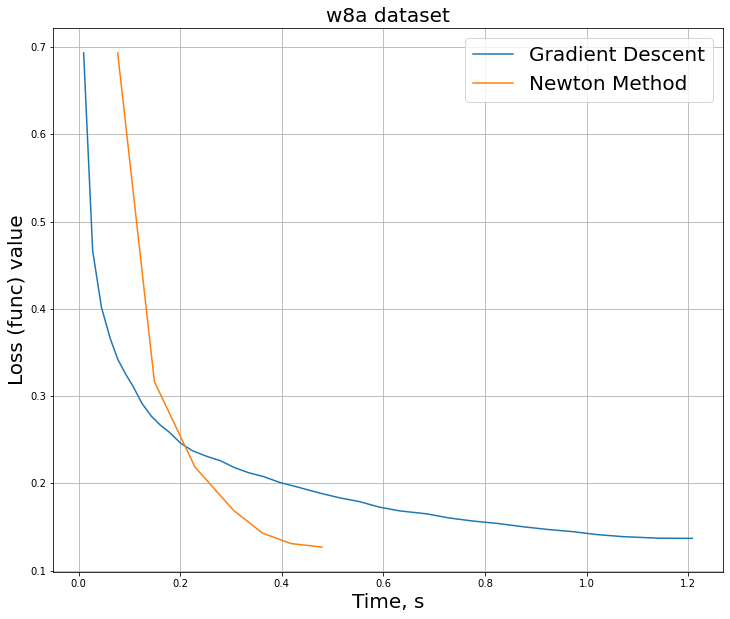
\includegraphics[height=7cm]{w8a_time.png}
	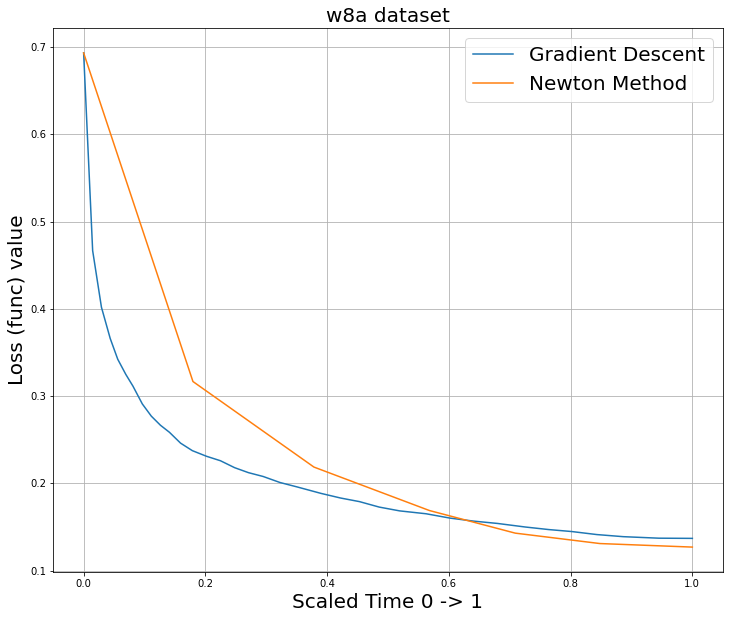
\includegraphics[height=7cm]{w8a_scale_time.png}
	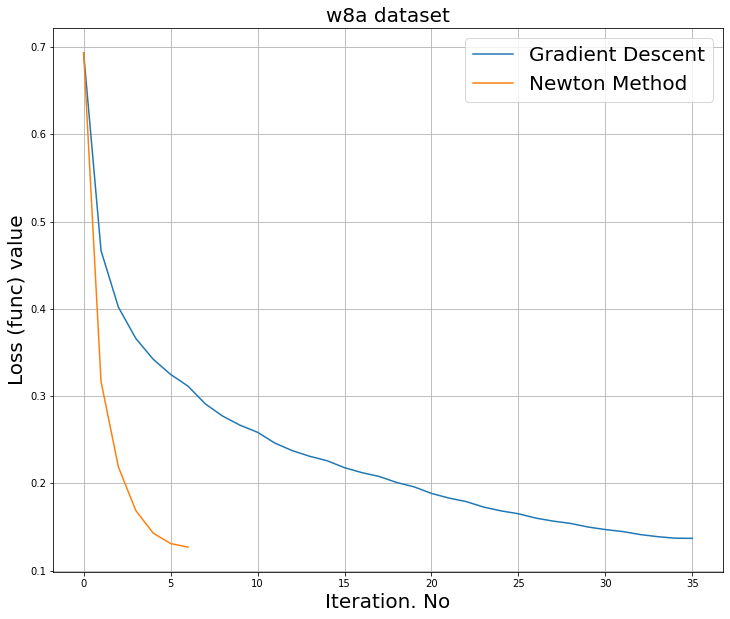
\includegraphics[height=7cm]{w8a_time_no.png}
\end{figure*}

 Видим, что в данном случае метод Ньютона оказался быстрее. Посмотрим на норму градиента.
 
 \\ \textbf{Note.} На одном из графиков перепутана подпись оси ординат.
 
 \begin{figure*}[h]
	\centering
	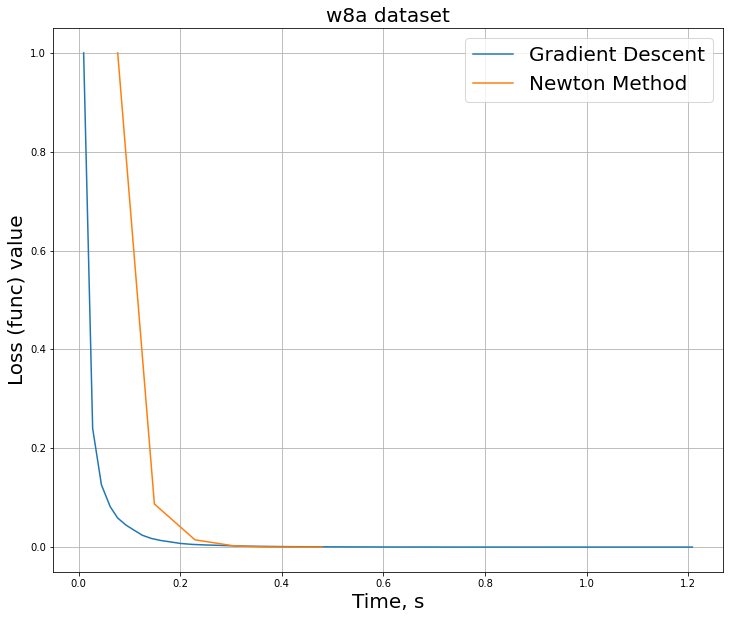
\includegraphics[height=6cm]{w8a_grad.png}
	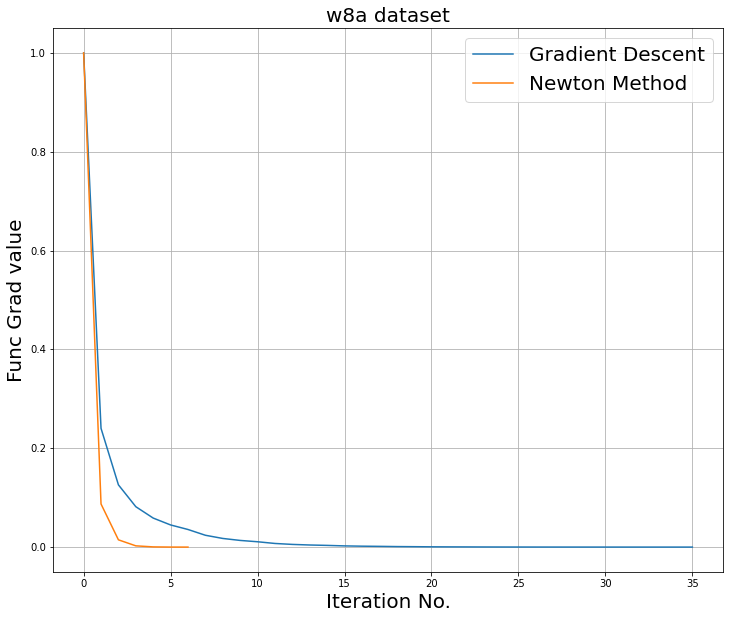
\includegraphics[height=6cm]{w8a_grad_no.png}
\end{figure*}

\newpage

\textbf{Датасет gisette}.

Зависимость значения функции от времени, от масштабированного времени (на отрезок $[0, 1]$), от номера итерации.


\begin{figure*}[h]
	\centering
	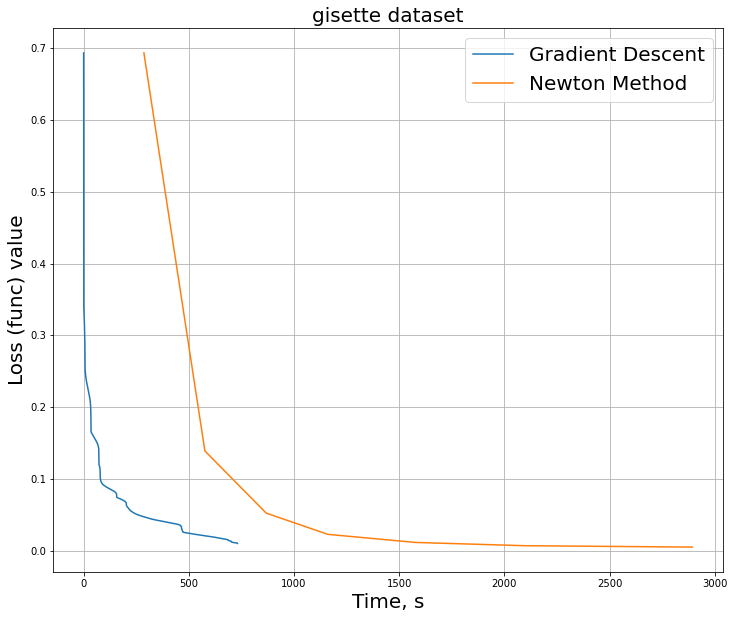
\includegraphics[height=7cm]{gisette_time.png}
	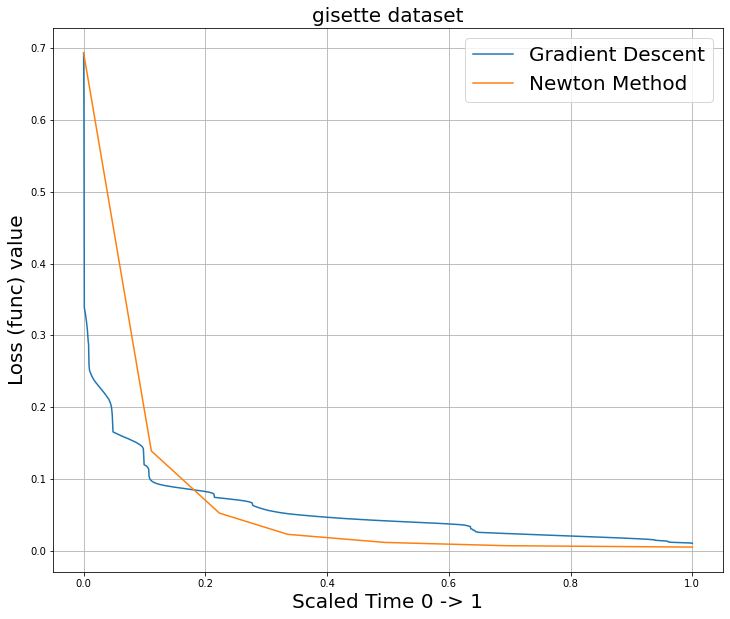
\includegraphics[height=7cm]{gisette_scale_time.png}
	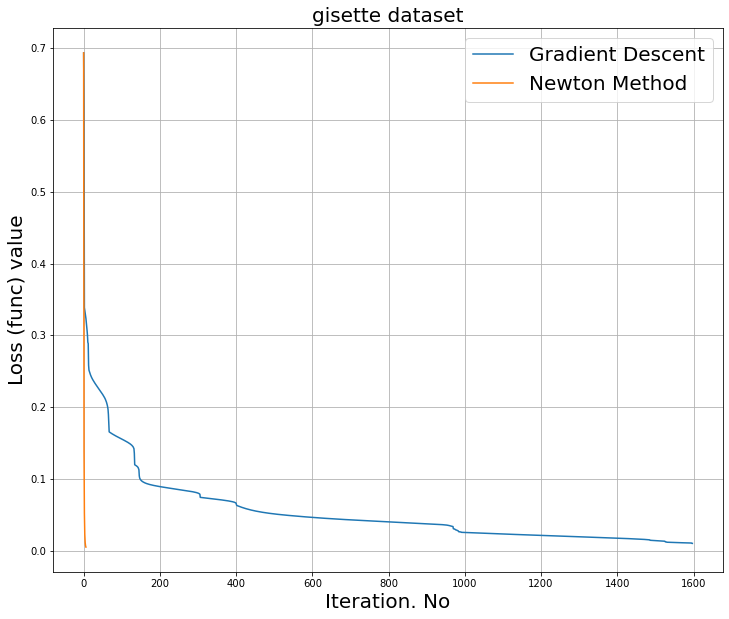
\includegraphics[height=7cm]{gisette_time_no.png}
\end{figure*}

В данном случае метод Ньютона оказался медленнее. Посмотрим на норму градиента.
 
 \\ \textbf{Note.} На одном из графиков перепутана подпись оси ординат.
 
 \begin{figure*}[h]
	\centering
	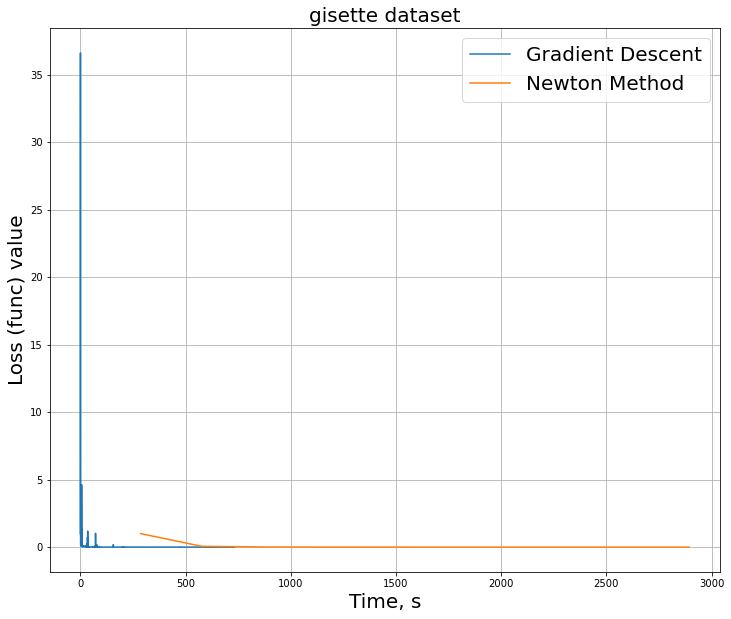
\includegraphics[height=6cm]{gisette_grad.png}
	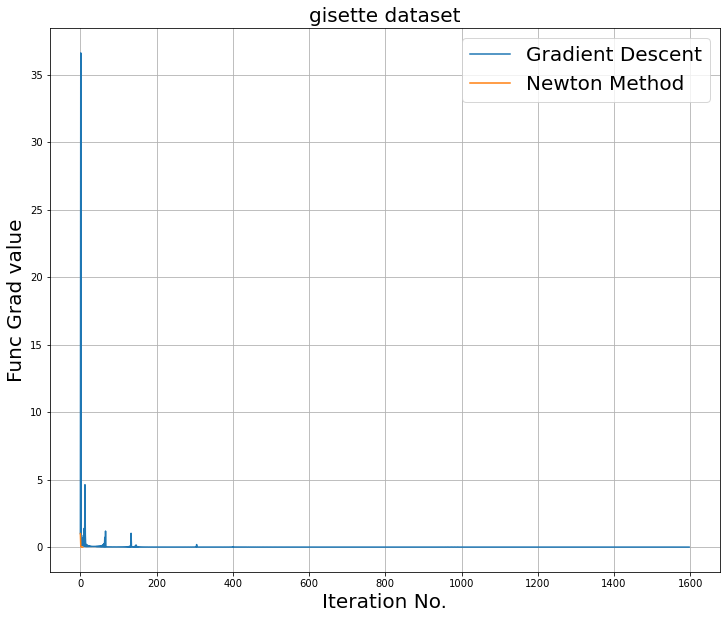
\includegraphics[height=6cm]{gisette_grad_no.png}
\end{figure*}

 По каким-то причинам методы долго бродили вокруг оптимальной точки, пытаясь в нее попасть.
 
 \newpage
 
 \textbf{Датасет real-sim}.

Зависимость значения функции от времени, от масштабированного времени (на отрезок $[0, 1]$), от номера итерации.


\begin{figure*}[h]
	\centering
	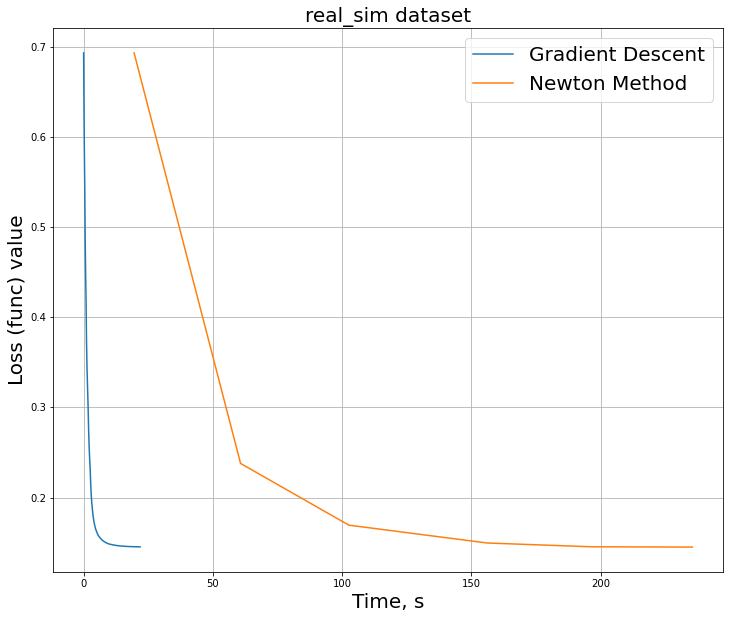
\includegraphics[height=7cm]{real_time.png}
	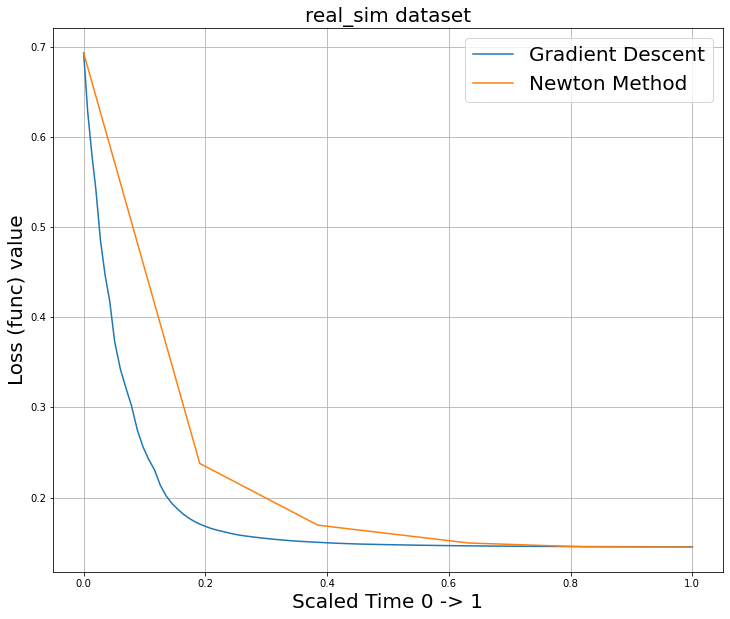
\includegraphics[height=7cm]{real_scale_time.png}
	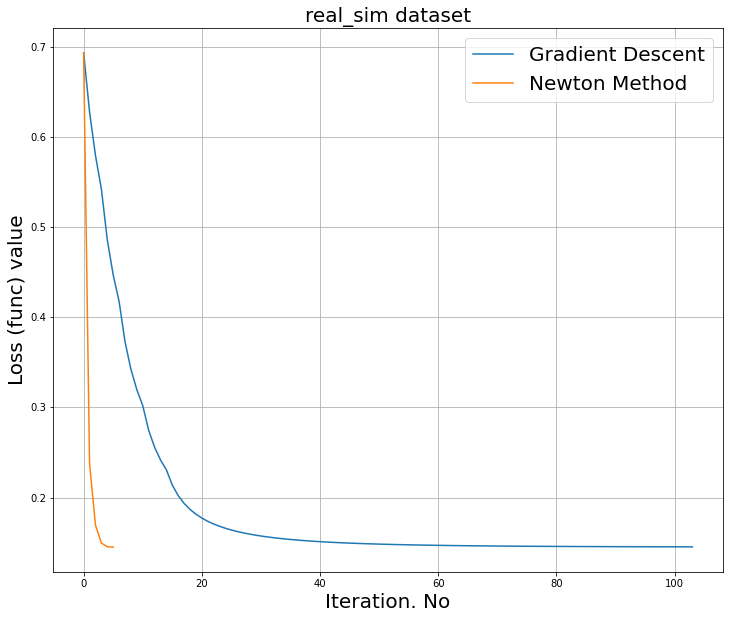
\includegraphics[height=7cm]{real_time_no.png}
\end{figure*}

В данном случае метод Ньютона оказался медленнее. Посмотрим на норму градиента.
 
 \\ \textbf{Note.} На одном из графиков перепутана подпись оси ординат.
 
 \begin{figure*}[h]
	\centering
	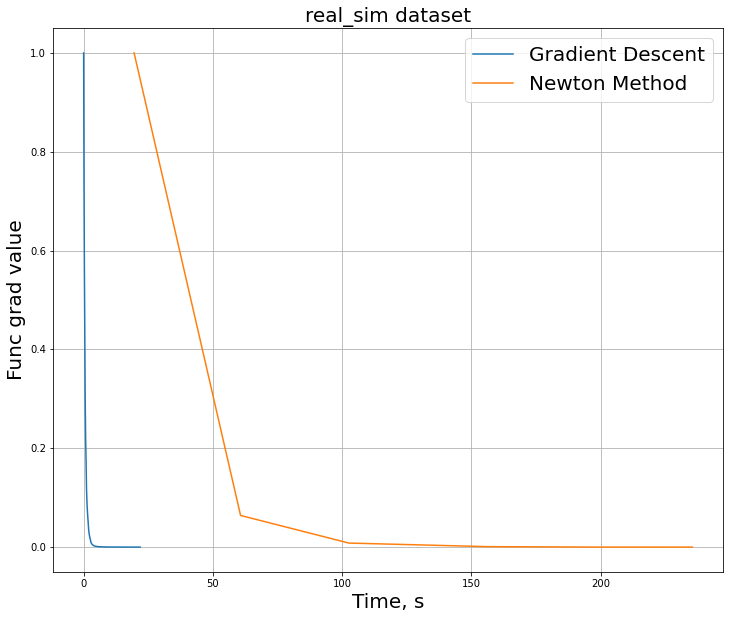
\includegraphics[height=6cm]{real_grad.png}
	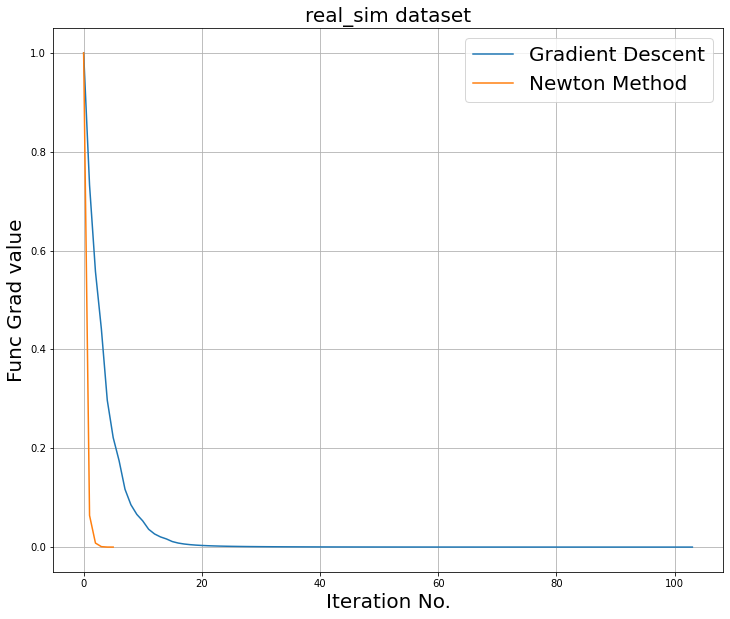
\includegraphics[height=6cm]{real_grad_no.png}
\end{figure*}

Видим, насколько быстрее метод Ньютона уменьшеает градиент, чем градиентный спуск.


\end{document}
